\section{Influenza Infection Prevention and Treatment}

Preventative measures, such as annual vaccination, hand washing, respiratory hygiene, and post exposure self-isolation are the best available measures in mitigating influenza infection risks \cite{influenza_seasonal_2018}.

Influenza vaccine formulation, recommended by WHO commonly includes \cite{RecommendedCompositionVaccines}

\begin{itemize}
    \item one H1N1 influenza A virus,
    \item one H3N2 influenza A virus,
    \item one or two influenza B viruses.
\end{itemize}

Influenza vaccine provides immunity to healthy adults even when formulation is not perfectly matched to circulating virus strains, but vaccination is especially important for individuals in high risk groups.

Likewise, in cases where disease occurs, for healthy adults WHO suggests symptomatic treatment and social distancing. For high risk groups the use of antiviral drugs is recommended \cite{influenza_seasonal_2018}. So far, two main classes of antiviral drugs against influenza have been developed (Figure \ref{figure:fluDrugs}).

Adamantane type drugs, such as amantadine, bind to M2 ion channel, preventing endosomal acidification, which inhibits virus uncoating. In 2011 WHO reported that the majority of circulating influenza A viruses are resistant to this type of drug \cite{whoAntivirals2011}. WHO no longer recommends adamantanes for use \cite{influenza_seasonal_2018}.

\begin{sidewaysfigure}
\begin{center}
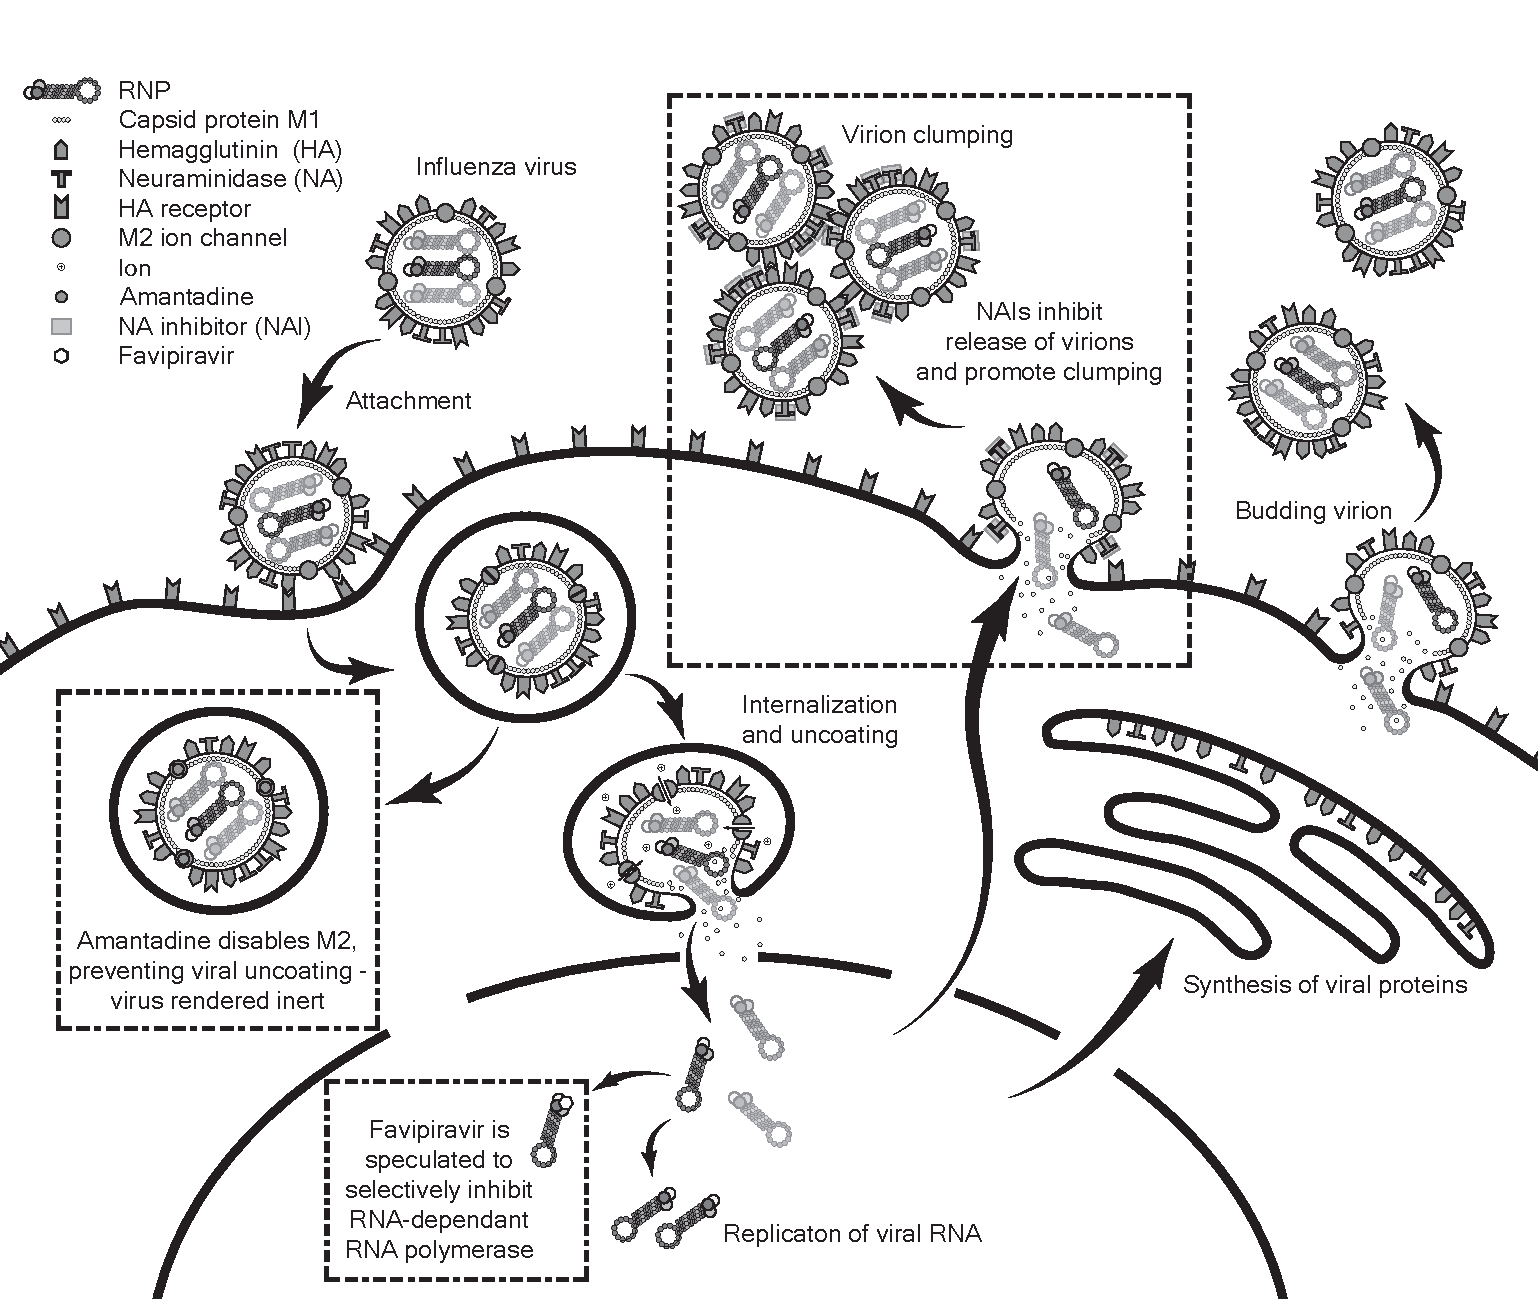
\includegraphics[width=0.75\textwidth, trim={0cm 0cm 0cm 0cm}, clip]{D_chapters/0_introduction/flu_drug.pdf}
\captionof{figure}{Mechanism of action of influenza antiviral drugs}
\label{figure:fluDrugs}
\end{center}
\end{sidewaysfigure}

Neuraminidase inhibitors bind to the viral surface enzyme neuraminidase and prevent cell surface receptor cleavage, inhibiting new virions' escape from infected cells. 2016-2017 survey reported that only about 0.2\% of collected influenza viruses showed resistance to one or more type of neuraminidase inhibitors \cite{lackenby2018global}. This type of drug remains suitable for use in the clinic, but emerging resistance makes continued monitoring necessary.

Additionally, favipiravir is a broad spectrum antiviral drug, which acts as a chain terminator at the site of viral RNA incorporation \cite{shiraki2020favipiravir}. Wide applicability to a variety of viruses often comes with concerns of cellular toxicity. Favipiravir has been approved as an emergency treatment for novel (rather than seasonal) influenza viruses in Japan in 2014, however wider approval is delayed in part due to potential teratogenic concerns.
